\section{Semilattice property}

\label{section-semilattice}

The aim of this section is to prove that $\Dyck_n$ is a lower
semilattice, namely any two elements have a meet. This will be done by
providing an explicit procedure to compute the meet of two elements
$a$ and $b$. At each step of this procedure, the pair $(a,b)$ is
replaced by another pair $(a',b')$ such that $(a',b')$ are strictly closer to
each other (in the sense of sharing a longer prefix) and the elements below both $a$ and $b$ are
exactly the elements below both $a'$ and $b'$. The procedure ends when $a$
becomes equal to $b$.

\subsection{Some technical lemmas}

This subsection proves several useful lemmas, that will be used in
\Cref{proof_semi} to describe the meet-building procedure.

Let us say that two elements $u$ and $v$ in $\Dyck_n$ share a prefix
of length $i$ if the first $i$ letters of $u$ are the same as the
first $i$ letters of $v$.

\begin{lemma}
  \label{forcer_un}
  Let $u \in \Dyck_n$, with a letter $0$ at position $i+1$. Consider
  the set $R_i(u)$ of elements $v \in \Dyck_n$ such that $u \leq v$,
  $u$ and $v$ share a prefix of length $i$ and $v$ has a letter~$1$ at
  position $i+1$.

  Either $R_i(u)$ is empty or $R_i(u)$ has a unique minimal element.
\end{lemma}
This will follow from \Cref{sub_forcer_un}.

Keeping the same notations, let us denote by $p$ (as \emph{prefix}) the first $i$ letters
of $u$. Then $u$ has a unique expression of the form
\begin{equation}
  \label{locked_pic}
  u = p \, 0^{\ell} \, X_0 0^{k_0} \, X_1 0^{k_1} \, \dots X_r 0^{k_r} \, X_{r+1},
\end{equation}
where for $j \leq r$ each $X_j$ is a non-empty Dyck path, $\ell > 0$,
all $k_j > 0$ and the final $X_{r+1}$ is any Dyck path (possibly
empty). This expression is obtained by starting after the prefix $p$ and
repeatedly doing the following : go down along the $0$ until reaching a
point before a letter $1$ (or final), then move on the path until reaching the
first point at the same height that is followed by a letter $0$ (or final).

%

Each of the $X_j$ is made of one or several blocks. Such a block is
\emph{unlocked} if it can be slid without changing the prefix, and
\emph{locked} otherwise.

In each $X_j$ for $j \leq r$, all the blocks but the last one are
unlocked. In the last Dyck path $X_{r+1}$, all the blocks are unlocked.

\begin{center}
  Here is a sketch: \includegraphics[width=4cm]{assets/locked-block-sketch.png}, with locked blocks darker.
\end{center}


If for every $j \leq r$, the Dyck path $X_j$ has only one block and
$X_{r+1}$ is empty, then there is no unlocked block in $u$. In this
case, the set $R_i(u)$ in the statement of \Cref{forcer_un} will be
empty. Indeed any cover relation not changing the prefix will keep the
shape of the expression~\eqref{locked_pic} fixed, so that no block
becomes unlocked and $X_0$ can never be slid.

Let us therefore from now on assume the contrary. In this case, let us
denote by $\rise_i(u)$ the element obtained from $u$ by sliding the
first block in the first $X_j$ that contains an unlocked block, up to
the height of the starting point of the last block of the previous
$X_{j-1}$ or up to the end of the prefix $p$ of $u$ if $j = 0$. In the
resulting Dyck path, there is an unlocked block inside $X_{j-1}$ if
$j > 0$.

This defines an operator $\rise_i$ that acts by sliding one unlocked block. One
will also need the operator $\rise^{(2)}_i$ defined similarly but
sliding the second available unlocked block.


\begin{lemma}
  \label{sub_forcer_un}
  Let $u \in \Dyck_n$, with a letter $0$ at position $i+1$. Let
  $v \in \Dyck_n$ such that $u \leq v$, $u$ and $v$ share a prefix of
  length $i$ and $v$ has a letter $1$ at position $i+1$. Then
  $\rise_i(u) \leq v$.
\end{lemma}

\begin{proof}
  The proof will use a decreasing induction (in the poset) on $u$
  among elements smaller than $v$ and sharing with $u$ the same prefix
  of length $i+1$.

  Since $u \leq v$, there must be an element $u'$ covering $u$ such
  that $u' \leq v$. Necessarily, $u'$ shares a prefix of length $i$
  with $u$ and $v$.

  It can happen that there is no such $u'$ sharing with $u$ a prefix
  of length $i+1$. This is the base case for the induction and it will
  just be taken care of below inside the case~\ref{sub2.1}. Otherwise, pick
  such an $u'$.

  \smallskip

  The possible such cover relations $u \leq u'$ can be classified into several types:
  \begin{enumerate}%
  \item\label{proof_lemma7.2_1} strictly inside one of the blocks of $X_k$ with $k \leq j$,
  \item\label{proof_lemma7.2_2} one block of $X_j$ is slid,
  \item\label{proof_lemma7.2_3} somewhere on the right of $X_j$.

  \end{enumerate}

  Let us first assume that there is a cover relation $u \leq u'$ of type~\eqref{proof_lemma7.2_1}
  with $u' \leq v$. In $u'$, one finds the same first unlocked block
  as in $u$. By induction, one also has $\rise_i(u') \leq v$. There
  is a sequence of cover relations $u \leq u' \leq \rise_i(u')$. But these
  cover relations commute, so that $\rise_i(u) \leq \rise_i(u')$.

  Let us now assume that there is a cover relation $u \leq u'$ of type~\eqref{proof_lemma7.2_3} with $u' \leq v$. In $u'$, one finds the same first unlocked
  block as in $u$, because this block is not the last block of
  $X_j$. By induction, one also has $\rise_i(u') \leq v$. There is a
  sequence of cover relations $u \leq u' \leq \rise_i(u')$. But these
  cover relations also commute, so that again
  $\rise_i(u) \leq \rise_i(u')$.

  There remains to assume that there is a cover relation $u \leq u'$
  of type~\eqref{proof_lemma7.2_2} with $u' \leq v$. There are three sub-cases.

  \begin{enumerate}[(2.\arabic{enumi})]
%
\setcounter{enumi}{2}
\item\label{sub2.3} 
  If the slid block $B$ is neither the
  first block nor the second block of $X_j$, then one can argue as in
  type~\eqref{proof_lemma7.2_3}, because the first unlocked block remains the
  first block of $X_j$, which is not affected.

\setcounter{enumi}{1}
\item\label{sub2.2} 
%
If the slid block $B$ is the second block of $X_j$, then either
  $X_j$ contains at least~$3$ blocks or the block $B$ is at the end of
  $u$, for otherwise $B$ is locked.  Then one can
  check directly that there is a cover relation
  $\rise_i(u) \to \rise_i(u')$. By induction, one also has $\rise_i(u') \leq v$.

  \begin{figure}[htb]
    \centering
    $u$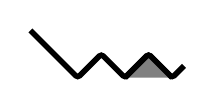
\begin{tikzpicture}[scale=.15]
      \draw[rounded corners=1, color=black, line width=2] (4, 4) -- (5, 3) -- (6, 2) -- (7, 1) -- (8, 0) -- (9, 1) -- (10, 2) -- (11, 1) -- (12, 0) -- (13, 1) -- (14, 2) -- (15, 1) -- (16, 0) -- (17, 1);
      \draw[rounded corners=1, color=black, fill=gray, line width=2] (12, 0) -- (13, 1) -- (14, 2) -- (15, 1) -- (16, 0);
    \end{tikzpicture}$\quad\phantom{\longrightarrow}\put(-15,5){$\longrightarrow$} \quad u'$
    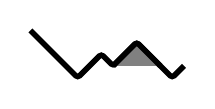
\begin{tikzpicture}[scale=.15]
      \draw[rounded corners=1, color=black, line width=2] (4, 4) -- (5, 3) -- (6, 2) -- (7, 1) -- (8, 0) -- (9, 1) -- (10, 2) -- (11, 1) -- (12, 2) -- (13, 3) -- (14, 2) -- (15, 1) -- (16, 0) -- (17, 1);
      \draw[rounded corners=1, color=black, fill=gray, line width=2] (11, 1) -- (12, 2) -- (13, 3) -- (14, 2) -- (15, 1) ;
    \end{tikzpicture}
    \caption{First blocks of $X_j$ for the case~\ref{sub2.2} in the proof of \Cref{sub_forcer_un}}
    \label{cas2.2}
  \end{figure}

\setcounter{enumi}{0}
\item\label{sub2.1} 
%
Assume now that the slid block $B$ is the first block of
  $X_j$. If $u' = \rise_i(u)$, the statement holds directly. This is
  what happens in the base case of the induction. Otherwise, the block
  $B$ can either be slid too high or too low compared to the exact
  height of the end of $X_{j-1}$ if $j > 0$, or too low compared to the end of the
  prefix $p$ of $u$. In both cases, it becomes (part of) a locked
  block. The existence of $v$ then forces that there is (in $u$ and $u'$) another
  unlocked block in $X_k$ for some $k \geq j$.

  If the first block $B$ of $X_j$ is slid too low in $u'$, one can
  apply repeatedly $\rise_i$ to $u'$ until this operator is sliding
  again the block $B$ itself. Let us call $u''$ the result. Starting
  from $X_k$ which contains the first unlocked block in $u'$, each
  $\rise_i$ unlocks the first block in the previous $X$. Then by
  induction, one has $u'' \leq v$. One can also see that
  $\rise_i(u) \leq u''$ by repeating on $\rise_i(u)$ all the same
  slidings performed from $u'$ to $u''$.

  The first block $B$ of $X_j$ can only be slid too high in $u'$ if
  $j > 0$, because otherwise the prefix would change. In this case,
  one can apply repeatedly $\rise_i$ to $u'$ until this operator is
  unlocking the block containing the slid block $B$ itself. Let us
  call $u''$ the result. Then by induction, one has $u'' \leq v$. Then
  one can apply the operator $\rise^{(2)}_i$ several times on
  $\rise_i(u)$ until making the slid block $B$ unlocked again. In
  other words, one replays on $\rise_i(u)$ all the sliding moves
  performed on $u'$, by replacing the action of $\rise_i$ by the
  action of $\rise^{(2)}_i$. Let us call the result $\bar{u}$. Then in $\bar{u}$,
  the block $B$ is unlocked and sliding this block (to the appropriate
  height) gives a cover relation $\bar{u} \to u''$. This implies that
  $\rise_i(u) \leq u''$.
\end{enumerate}

  In all cases, one obtains that $\rise_i(u) \leq v$.
\end{proof}

\begin{proof}
Let us now give the proof of \Cref{forcer_un}. 

One can assume that $R_i(u)$ is not empty. Let us pick any $v$ in $R_i(u)$.

Then one can iterate \Cref{sub_forcer_un}, which when applied to the
pair $(u,v)$ gives another pair $(\rise_i(u),v)$ that satisfies the
same hypotheses as long as $j > 0$. At each step, the index $j$ of
$x_j$ containing the first unlocked block in $u$ is decreased by
one. In the last step, when $j=0$, the element $\rise_i(u)$ becomes an
element $w$ of $R_i(u)$ such that $w \leq v$.

Because the construction of $w$ is an iteration of $\rise_i$ applied
to $u$, it does not depend on $v$. Therefore $w$ is smaller than any
element of $R_i(u)$. Uniqueness of such a global minimum is clear.
\end{proof}

%

For $v,w$ in $\Dyck_n$, let $M(v,w)$ be the set of Dyck paths that are
smaller than both $v$ and $w$. This set is never empty.

\begin{lemma}
  \label{meet_with_prefix}
  Let $v$ and $w$ in $\Dyck_n$ that share a prefix of length $i$. Then
  for every element $u$ in $M(v,w)$, there exists $u'$ in $M(v,w)$
  such that $u \leq u'$ and $u'$ shares a prefix of length $i$ with $v$
  and $w$.
\end{lemma}
\begin{proof}
  By induction on $i$. This is true for $i=1$, for $u'=u$. Assume now
  that $v$ and $w$ share a prefix of length $i+1$ and let $u'_i$
  be defined by induction hypothesis for the shorter common prefix of
  length $i$. If the last letter in the common prefix of length $i+1$
  is the same as the letter of $u'_i$ at position $i+1$, one can take
  $u'$ to be $u'_i$.

  Because $u'_i \in M(v,w)$, there remains only the case where the
  letter of $u'_i$ at position $i+1$ is $0$ and the last letter in the
  common prefix of length $i+1$ of $v$ and $w$ is $1$. Let us apply
  \Cref{forcer_un} to $u'_i$. The set $R_{i}(u'_i)$ is not empty as
  it contains $v$ and $w$. One can therefore take $u'$ to be its unique
  minimal element.
\end{proof}

\subsection{Proof of semilattice property}

\label{proof_semi}

Let us start with more lemmas.

Let $w$ be a Dyck path such that the $i$-th step in $w$ is $1$ and
this step does not start at height $0$.  On the right from the start
$i_0$ of $i$-th step, move on the path $w$ until meeting a point $i_1$
at the same height and followed by a $0$ step. This must happen, as
the height of $i_0$ is not zero. Between $i_0$ and $i_1$, there is in
$w$ a non-empty sequence of block-indecomposable subpaths $x_1, \dots, x_N$.

Let us define another Dyck path $\des_i(w)$ by sliding down in $w$ the
subpath $x_N$ as much as possible, namely by exchanging $x_N$ with all
the consecutive $0$ steps on its right. Then there is a cover relation
$\des_i(w) \to w$ that is sliding the subpath $x_N$ up.

\begin{lemma}
  \label{sub_force_0}
  Let $w$ be a Dyck path such that the $i$-th step in $w$ is $1$ and
  this step does not start at height $0$. Let $u \leq w$ such that the
  $i$-th step in $u$ is $0$ and $u$ and $w$ share a prefix
  of length $i - 1$. Then $u$ is smaller than $\des_i(w)$.
\end{lemma}
\begin{proof}
  The proof will be by increasing induction (in the poset) on $w$
  among elements larger than $u$ and sharing with $u$ the same prefix
  of length $i - 1$.

  Since $u \leq w$, there exists $w'$ covered by $w$ such that
  $u \leq w'$. Necessarily, $w'$ shares the same prefix of length
  $i-1$ with $u$ and $w$.

  It can happen, in the base case of the induction, that there is no
  such $w'$ that shares with $w$ a prefix of length $i$. Then it must
  be the case that $N=1$ and $w' = \des_i(w)$.

  If $w' = \des_i(w)$, the statement clearly holds.

  Because of the shared prefix, the other possible down-sliding moves
  from $w$ are of three types, according to the slid subpath $x$:
  \begin{enumerate}%
  \item\label{proof_lemma7.4_1} $x$ is inside one of the $x_j$, not ending in the final
    sequence of $0$ of $x_j$,
  \item\label{proof_lemma7.4_2} $x$ is inside one of the $x_j$, ending in the final
    sequence of $0$ of $x_j$,
  \item\label{proof_lemma7.4_3} $x$ is somewhere on the right of $x_N$.
  \end{enumerate}

  In type~\eqref{proof_lemma7.4_1}, $x_j$ is replaced by another block-indecomposable
  subpath. In type~\eqref{proof_lemma7.4_2}, if $j < N$, then $x_j$ is replaced by (split
  into) two block-indecomposable subpaths.

  Assume first that $u \leq w'$ where $w' \to w$ is of type~\eqref{proof_lemma7.4_3}. By
  induction, $u \leq \des_i(w')$. There is a chain of cover relations
  $\des_i(w') \to w' \to w$. These two cover relations commute if the slid
  subpath in the sliding move $w' \to w$ is not the first subpath after
  $x_N$. Otherwise, one can find a chain of two cover relations from
  $\des_i(w')$ to $\des_i(w)$. In all cases,
  $\des_i(w') \leq \des_i(w)$.

  Assume now that $u \leq w'$ where $w' \to w$ is of type~\eqref{proof_lemma7.4_1}. By
  induction, $u \leq \des_i(w')$. There is a chain of cover relations
  $\des_i(w') \to w' \to w$. These cover relations commute, and therefore
  $\des_i(w') \leq \des_i(w)$.

  Assume then that $u \leq w'$ where $w' \to w$ is of type~\eqref{proof_lemma7.4_2}. By
  induction, $u \leq \des_i(w')$. There is a chain of cover relations
  $\des_i(w') \to w' \to w$. If $j < N - 1$, these cover relations
  commute, and therefore $\des_i(w') \leq \des_i(w)$.

  If $j = N$, then one can apply twice the induction step to obtain that
  $u \leq \des_i(\des_i(w'))$. But $\des_i(\des_i(w')) \leq \des_i(w)$
  because one can split $x_N$ after it has been slid down.

  If $j = N-1$, one can also apply twice the induction step, to get
  that $u \leq \des_i(\des_i(w'))$. One then checks that
  $\des_i(\des_i(w')) \leq \des_i(w)$ holds also in this case, by just
  one cover relation.

  One therefore deduces the statement in all cases.
\end{proof}

Keeping the same notations, let $s_i(w)$ denote $\des_i^N(w)$, the
image of $w$ under the $N$-times iteration of the application
$\des_i$.

\begin{lemma}
  \label{force_0}
  Let $w$ be a Dyck path such that the $i$-th step in $w$ is $1$ and
  this step does not start at height $0$. Let $S_i(w)$ be the set
  of all Dyck paths $u$ such that $u \leq w$, the $i$-th letter of $u$
  is $0$ and $u$ and $w$ share the same prefix before the $i$-th letter.
  Then $s_i(w)$ is the unique maximal element of $S_i(w)$.
\end{lemma}
\begin{proof}
  First note that $s_i(w)$ is indeed in $S_i(w)$.

  Let $u$ be an element of $S_i(w)$. One can apply \Cref{sub_force_0}
  to the pair $(u,w)$ to get another pair $(u, w')$ where
  $w'=\des_i(w)$. Either $w' = s_i(w)$, or this new pair satisfies
  again the hypotheses of \Cref{sub_force_0}. One can therefore repeat
  this exactly $N$ times, until reaching the pair $(u,s_i(w))$. In
  particular, $u \leq s_i(w)$.
\end{proof}


\begin{theorem}
  The poset $(\Dyck_n, \sm)$ is a meet-semilattice.
\end{theorem}
\begin{proof}
  Let $v$ and $w$ be two Dyck paths, and let us look for their
  meet. One can assume that $v$ and $w$ are not equal.

  Start from the left, until meeting a difference between $v$ and
  $w$. Let $i$ be the last common point. One can assume that $w$ is
  above $v$ just after the point $i$, by exchanging $v$ and $w$ if
  necessary. Note that the height of $i$ cannot be zero.

  One can therefore apply \Cref{force_0} to $w$ for the step after
  position $i$, and obtain an element $w'$ which is maximal among all
  elements smaller than $w$ that share the same prefix followed by
  the letter $0$.

  This gives a new pair of elements $(v,w')$ with $w' \leq w$. Let us
  prove that $M(v,w) = M(v,w')$. The inclusion $M(v,w') \subseteq
  M(v,w)$ is clear because $w' \leq w$.

  Conversely, let $u$ be an element of $M(v,w)$. Using
  \Cref{meet_with_prefix}, one can find $u'$ in $M(v,w)$ with $u \leq
  u'$ and $u'$ share the common prefix of $v$ and $w$. Note that the
  first letter after the common prefix in $u'$ is $0$, because $u'
  \leq v$. It therefore follows from the definition of $w'$ that $u'
  \leq w'$.

  Hence $M(v,w) = M(v,w')$, and the common prefix of $v$ and $w'$ is
  strictly longer. Therefore iterating this whole procedure on pairs
  of Dyck paths ends at a common Dyck path $z$, that is smaller than
  $v$ and $w$ and such that $M(z,z) = M(v,w)$. This $z$ is therefore
  the meet of $v$ and $w$.
\end{proof}
